\documentclass[12pt]{scrartcl}
\usepackage[utf8]{inputenc}
 \usepackage{fancyhdr, graphicx}
 \usepackage[german]{babel}
 \usepackage[scaled=0.92]{helvet}
 \usepackage{enumitem}
 \usepackage{parskip}
 \usepackage{lastpage} % for getting last page number
\usepackage{listings}
\usepackage{caption}
\usepackage{color}
\usepackage{xcolor}
\DeclareCaptionFont{white}{\color{white}}
\DeclareCaptionFormat{listing}{\colorbox{gray}{\parbox{\textwidth}{#1#2#3}}}
\newcommand\Fontvi{\fontsize{6}{7.2}\selectfont}

 \renewcommand{\familydefault}{\sfdefault}
 
 \fancypagestyle{firststyle}{ %Style of the first page
 \fancyhf{}
 \fancyheadoffset[L]{0.6cm}
 \lhead{
 
\includegraphics[scale=0.8]{./FHNW_HT_10mm.jpg}}
 \renewcommand{\headrulewidth}{0pt}
 \cfoot{Thomas Baumann \& Egemen Kaba}
}

\fancypagestyle{documentstyle}{ %Style of the rest of the document
 \fancyhf{}
 \fancyheadoffset[L]{0.6cm}
\lhead{
 
\includegraphics[scale=0.8]{./FHNW_HT_10mm.jpg}}
 \renewcommand{\headrulewidth}{0pt}
 \lfoot{Laborübung 2}
 \cfoot{Thomas Baumann \& Egemen Kaba}
 \rfoot{\thepage\ / \pageref{LastPage} }
}

\pagestyle{firststyle} %different look of first page
 
\title{ %Titel
Applikationssicherheit 
\vspace{0.2cm}
}

 \begin{document}
 \maketitle
 \thispagestyle{firststyle}
 \pagestyle{firststyle}
 \begin{abstract}
 \begin{center}
 Laborübung 2
 \end{center}
 \vspace{0.5cm}
\hrulefill
\end{abstract}

 \pagestyle{documentstyle}
 \tableofcontents
 \pagebreak
 
\section{Architektur}
Die Architektur ist wie in Abbildung \ref{fig:Arch} implementiert. Dabei haben wir uns an das MVC-Pattern gehalten, damit die Rechte klar getrennt werden.

Sämtliche Anfragen des Client-Browsers werden von einem Servlet entgegengenommen, welches auf einem Tomcat Server läuft. Dieses reicht die Anfragen entsprechend dem page-Parameter und GET bzw. POST die entsprechende Methode des Controllers weiter. Der Controller erstellt, wenn benötigt, ein Objekt der Klasse Company, dem Model, indem er entweder die erhaltenen Daten in eine neu Instanz abfüllt oder mithilfe des CompanyDAO auf die Datenbank zugreift, um von diesem ein Objekt zu erhalten. Über das DAO kann dementsprechend auch ein Company-Objekt gespeichert, bzw. nachgeführt werden. Als Datenbanksystem wird MySQL verwendet. Mit Hilfe des HttpServletRequest werden JavaServer Pages gerendert und als Antwort zurück an den Client gesendet, bzw. über den HttpServletResponse wird eine Weiterleitung ausgelöst.
\begin{figure}
	\centering
	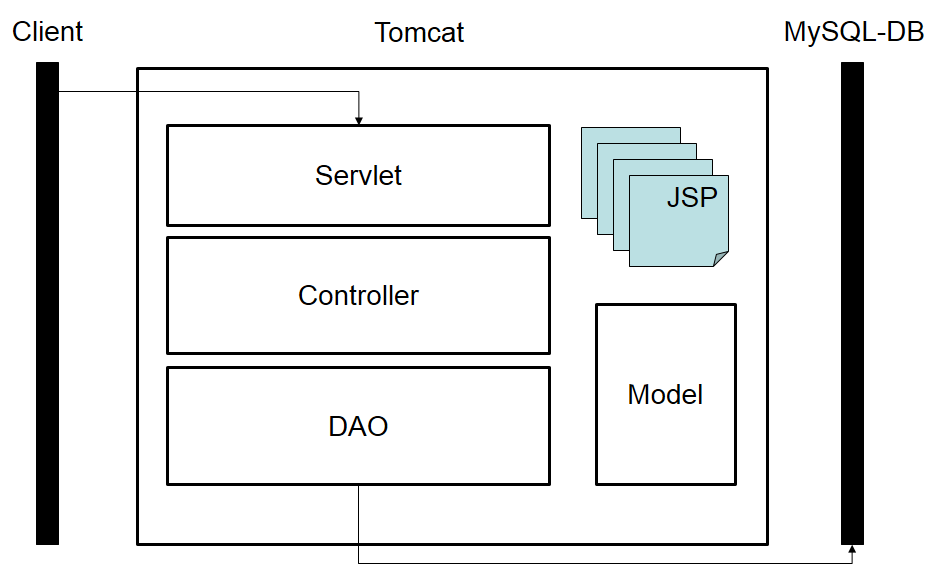
\includegraphics[width=12cm]{./Architektur.png}
	\caption{Architektur}
	\label{fig:Arch}
\end{figure}

\section{Ressourcen}
\textbf{JavaServerPages}\newline
Als View-Schicht werden JavaServerPages verwendet, mit Hilfe deren auch normaler Java-Code ausgeführt werden kann. Der Java Code wird für das anzeigen der Fehler- bzw. Erfolgsmeldungen und der Daten aus der Datenbank / Model verwendet.

Die vom Benutzer eingegebenen Werte in Formularen (POST-Daten) sind implizit in einer Map abgelegt, welche unter dem Namen "param" abrufbar ist. So kann zum Beispiel das Feld "`name"' mit "`\$\{param.name\}"' ausgelesen werden.

Damit die JSP-Seiten nicht direkt aufgerufen werden können, sind sie im WEB-INF Verzeichnis des Tomcat Servers abgelegt.

\textbf{config.properties}\\
In dieser Java Property Datei sind die Konfigurationen für das E-Mail-Konto, den Zugriff auf die Datenbank und das Template für die Email abgespeichert. So können diese Einstellungen verändert werden, ohne dass der Code neu kompiliert werden muss.

\textbf{web.xml}\\
Da wir die Servlet Spezifikation Version 3.0 verwenden, kann das Servlet als WebServlet annotiert werden und auch der Security Constraint (Deklaration dass HTTPS verwendet werden muss) kann als Annotation festgelegt werden. Somit muss im Deployment Descriptor bloss das Welcome-File (Startseite) und die Konfiguration der Fehlerseiten definiert werden.

\textbf{database.sql}\\
Mit dieser Datei kann die Datenbank für die Applikation aufgesetzt werden. Dabei werden sowohl die benötigte Datenbank, die Tabelle mit den Spalten, als auch ein Benutzer mit den benötigten Berechtigungen erstellt.

\textbf{https-einrichten.txt}\\
In dieser Datei wird beschrieben, wie https auf einem Tomcat Server aufgesetzt werden kann.

\textbf{build.xml}\\
Das Ant Script automatisiert das Builden und das Deployment auf den Tomcat Server.

\section{Klassen}
Implementierungsdetails siehe Sourcecode.

\textbf{RattleBitsServlet}\\
Diese Klasse erbt von HttpServlet, ist somit die Schnittstelle der Applikation zur Aussenwelt.\\
In diesem Servlet wird im Konstruktor der Controller, der MailHelper sowie die Datenverbindung aufgesetzt. Hier wird ebenfalls auf GET- und POST-Anfragen reagiert. Beim Zerstören des Servlets wird ebenfalls darauf geachtet, dass abhängige Objekte sauber aufgeräumt werden.\\

\textbf{Controller}\\
Der Controller verarbeitet Anfragen, die an den Servlet gesendet wurden. Dabei prüfen die Methoden jeweils als erstes, ob der Benutzer bereits eingeloggt ist. Das Resultat dieser Anfrage wird benutzt, um festzustellen, ob der Benutzer die gewünschte Aktion durchführen kann, oder auf eine andere Seite weitergeleitet werden soll.\\
Da diverse Aktionen einen Zugriff auf die Datenbank voraussetzen, wird im Konstruktor ein Data Access Object, das CompanyDAO, mit der übergebenen Connection instanziert.\\
Das Weiterleiten auf Seiten, wird über den RequestDispatcher geregelt. Die Strings, welche Standorte der Views angeben sind dabei als Konstanten definiert.\\
Im Controller wird ebenfalls die Koordination zwischen diversen Komponenten, wie diversen Helpern und Utilities, mit der Applikation vorgenommen.

\textbf{CompanyDAO}\\
Das CompanyDAO ist die Schnittstelle der Applikation zur Datenbank. im Konstruktor wird deshalb auch ein Connection-Objekt übergeben, in dem Informationen enthalten sind, die für die Verbindung zur Datenbank notwendig sind.\\
In dieser Klasse werden einige Methoden bereit gestellt, welche Objetke des Models in der Datenbank persistieren, oder mit Informationen aus der Datenbank instanzieren und zurückgeben sollen.\\
Die Abfragen zur Datenbank werden dabei mittels PreparedStatements ausgeführt.\\

\textbf{Company}\\
Diese Klasse stellt das Model dar. Diese Klasse enthält Informationen, die aus der Datenbank stammen, oder in der Datenbank persistiert werden sollen. Sie bietet zudem Methoden an, um die enthaltenen Daten per RegEx zu validieren.\\

\textbf{MailHelper}\\
Im MailHelper werden die Properties in config.properties ausgelesen, um eine Message zu präparieren und zu senden.\\

\textbf{Utility}\\
In der Utility werden zentral statische Methoden angeboten, die an mehreren Stellen in der Applikation verwendet werden. Diese sind im Detail eine Methode zum generieren eines randomisierten Strings gemäss der Passwort-Validations-Methoden sowie eine Methode, um Strings mittels SHA-256 zu hashen.\\

\textbf{Verifiers}\\
Die Methoden dieser Klasse, haben die Aufgabe eine PLZ zu verifizieren. Damit die Verifikation nicht auf einen einzelnen Webdienst gestützt ist, wird zuerst versucht auf post.ch zu verifizieren. Schlägt diese Verifikation aufgrund von Verbindungsproblemen fehl, wird die PLZ auf postleitzahlen.ch verifiziert.\\
Bei beiden Varianten kann die PLZ als Parameter in der URL angegeben werden. Die Antwort ist eine HTML-Page. Diese wird auf eine Meldung überprüft, welche darauf hindeutet, dass der Webdienst diese PLZ nicht gefunden hat.

\section{Sicherheitsmechanismen}
\subsection{Benutzereingaben}
In der ersten Sicherheitsstufe werden HTML-Zeichen bereits in der View escaped. Dies wird dadurch erreicht, dass JSTL (Java ServerPages Template Language) ein Tag anbietet, welches eine Benutzereingabe als Information kennzeichnet, welches in weiteren Schritten von weiteren Komponenten beansprucht wird.\\
Die zweite Sicherheitsstufe wurde im Model implementiert. Dort werden sämtliche Benutzereingaben validiert bevor sie weiter verwendet werden. Die Validation erfolgt durch Regular Expressions, welche von der Aufgabenstellung vorgegeben wurden.\\
Der dritte Schritt erfolgt vor dem Persistieren der Benutzereingaben in der Datenbank. Im CompanyDAO werden Benutzereingaben über PreparedStatements in der Datenbank gespeichert. Somit kann sicher gestellt werden, dass Informationen in der Datenbank garantiert sauber sind.\\
Beim Anzeigen der Informationen aus der Datenbank werden keine Sicherheitsmassnahmen getroffen, da davon ausgegangen wird, dass dank der zahlreichen Massnahmen beim Speichern, die Werte in der Datenbank garantiert sauber sind. Dadurch kann auch sichergestellt werden, dass SQL-Injection bzw. XSS-Attacken abgefangen werden können.\\
Auf spezielle Benutzereingaben wie der E-Mail und der PLZ wird in seperaten Kapiteln eingegangen.

\subsection{E-Mail}
Die E-Mail-Validierung wurde durch die Klasse E-Mail-Validator im Package org.apache.commons gelöst. Dieser implementiert eine genügend gute Lösung, um die meisten E-Mails validieren zu können. Eine andere Möglichkeit wäre gewesen den RegEx-String zu kopieren, der von http://www.ex-parrot.com/~pdw/Mail-RFC822-Address.html beschrieben wird. Diese Lösung implementiert den RFC822-Standard und wurde von einem Perl-Modul generiert. Wir haben uns jedoch auf eine rein Java-basierte Lösung entschieden, welches gewartet und auf dem neuesten Stand gehalten wird.\\
Die E-Mail-Verifizierung konnte nicht implementiert werden. Wir haben keine Lösung gefunden, welcher eine 100\% Verifizierung einer E-Mail-Adresse erlaubt hätte. Das Hauptproblem bestand darin, dass die meisten Mail-Server eine Antwort auf die E-Mail-Verifikation per Default verweigern. Dies ist auch verständlich, da sonst Spammer diese Information für ihre Zwecke ausnutzen könnten.\\
Das Versenden von E-Mails werden über das Package javax.mail.* in einem Helper gelöst.

\subsection{PLZ}
Die PLZ-Validierung wird wie die restlichen Benutzereingaben per RegEx validiert.\\
Die PLZ-Verifizierung erfolgt durch zwei Webdienste. Der erste Webdienst, der angesteuert wird, ist derjenige von post.ch. Gibt es bei der Verbindung zu diesem Webdienst ein Problem, wird auf den Webdienst von postleitzahlen.ch zurückgegriffen. Bei beiden Varianten können Parameter über die URL verschickt werden. Die Antwort wird anschliessend auf ein Stichwort untersucht, welches indiziert, dass die PLZ nicht gefunden wurde. Durch die zwei Webdienst wird sichergestellt, dass die Verfügbarkeit möglichst auf einem hohen Level gehalten werden kann.

\subsection{HTTPS}
\textbf{In Tomcat}\\
Die Installation von HTTPS haben wir wie folgt gelöst:
\begin{itemize}
	\item Generieren eines Keystores mittels keytool
	\item Suchen des Eintrags für den Connector mit dem Port 8443 in conf/server.xml vom Tomcat
	\item Ergänzen dieses Eintrags durch die Attribute keystoreFile, welches den Standort des Keystores angibt, und keystorePass, welches das Passwort des Keystores angibt.
\end{itemize}
Eine detaillierte Beschreibung ist im rsc-Ordner der Applikation zu finden.\\
Nach der Installation ist ein Keystore generiert, sowie der Connector, welches für HTTPS zuständig ist, konfiguriert worden, so dass dieser den Keystore verwendet wird.\\
In der Applikation wird im File web.xml ein SecurityConstraint für eine Web-Ressource mit einem User-Data-Constraint erstellt. Als Web-Ressource wurde die gesamte Applikation und als User-Data-Constraint CONFIDENTIAL definiert worden. Dies bedeutet, dass Tomcat automatisch auf HTTPS umstellt, wenn eine Seite der Applikation aufgerufen wurde. Mit dieser Lösung können wir jedoch nicht erst beim Login auf HTTPS umstellen, da der SecurityConstraint keine URL-Parameter, auf denen die Navigation aufbaut, unterstützt. Diese Lösung hat aber den Vorteil, dass sämtliche Kommunikation mit der Applikation über HTTPS erfolgt, was aus unserer Sicht die Sicherheit erhöht.\\
Eine weitere Lösungsmöglichkeit wäre gewesen, Filter zu implementieren. Bei Filtern müsste jedoch manuell implementiert werden, auf welchen Seiten eine Umstellung auf HTTPS nötig gewesen wäre. In der momentanen Lösung kann durch ein SecurityConstraint in einem File, welches für die Konfiguration von Tomcat gedacht ist, diese Umstellung definiert und bei Änderungen zentral und einfach geändert werden.

\subsection{Bedrohungsmodell Datenbank}
Falls die Applikation lokal betrieben wird, kann die Datenbank leicht geschützt werden, in dem die Datenbank im lokalen Modus konfiguriert ist, also keine Anfragen von ausserhalb beantwortet.\\
Falls die Applikaiton online betrieben wird, kann die Datenbank so konfiguriert werden, dass sie nur auf bestimmte IP-Adressen antwortet. Dies wäre die IP-Adresse des Servers, auf dem Tomcat läuft.\\
Eine weitere Bedrohung stellt SQL-Injection dar. Dies wird jedoch durch die diversen Sicherheitsmechansimen, die im Kapitel über Benutzereingaben beschrieben werden, verunmöglicht.

\subsection{Strategie Login-Versuche}
Unsere Strategie für mehrmalige falsche Login-Versuche umfasst eine Liste, die im Controller verwaltet wird. Diese Liste wird bei jedem Login-Versuch ergänzt. Diese Liste speichert in jedem Eintrag, welcher Nutzer, identifiziert durch den Benutzernamen, sich einloggen wollte, der wievielte Versuche es war und einem Zeitstempel, wann er zuletzt probiert hat, sich einzuloggen.
Ab einer gewissen Anzahl von Versuchen wird der Benutzer für weitere Versuche gesperrt und bekommt eine Meldung angezeigt.\\
Eine private finale Variable wird erstellt, um zu definieren, nach welcher Zeit ein Benutzer wieder einen Versuch hat sich einzuloggen. Bei einem Eintrag in der Liste wird überprüft, ob der Zeitstempel + diese Variable in der Zukunft liegt. Falls ja, wird der Counter für die Versuche raufgezählt, falls nicht, wird der Eintrag in dieser Liste gelöscht.\\

\subsection{Login und Identifikation}
Der Benutzername wird aus dem Firmennamen, sowie einer fortlaufenden Zahl generiert.\\
Das Passwort ist ein randomisierter String, welches zuerst per SHA-256 gehasht und später in HEX konvertiert wird. Die Konvertierung erhöht die Sicherheit des Passworts nochmal, falls ein Angreifer diesen knacken will. Der Benutzer erhält den randomisierten String. In der Datenbank wird das gehashte und konvertierte Passwort gespeichert.\\
Bei erfolgreichem Login, wird dem User eine Id zugewiesen. Dieser entspricht der Id in der Datenbank, welche bei der Registrierung einer Firma angelegt wird. Zusätzlich wird dem User ein randomisierter String zugewiesen, welcher während dem Login in der Datenbank gespeichert wird. Beide Informationen werden in der Session des Nutzers gespeichert.\\
Mit diesen Informationen kann fest gestellt werden, ob der Nutzer eingeloggt ist und ob dieser Nutzer, Informationen in der Session manipuliert hat. Denn ist die Kombination aus Id und String nicht in der Datenbank vorhanden, wird dem Nutzer die Zugriff auf weitere Seiten innerhalb des geschützten Bereichs verweigert.

\subsection{Interne Fehler}
Treten jegliche Fehler innerhalb des Servlets auf, welche von der Applikation verursacht worden sind, werden diese nicht an den Benutzer direkt weitergeleitet. Ein Mapping im File web.xml verweist bei einer Fehlermeldung auf eine eigene Fehlerseite. Diese Massnahme wurde getroffen, damit der Benutzer keine Informationen über Fehler in der Ausführung der Applikation erhalten kann, welche allfällige konkrete Implementierungsdetails verraten. Durch das mappen auf einen universellen Fehlercode wird zudem sicher gestellt, dass auch in Zukunft diese Weiterleitung funktioniert und nicht durch neuere Versionen ausgehebelt wird.


\end{document}